\documentclass[12pt,a4paper]{article}

% === PAQUETES === (((
\usepackage{amsmath}
\usepackage[shortlabels]{enumitem}
\usepackage{amsfonts}
\usepackage{ragged2e}
\usepackage{subfigure}
\usepackage{amssymb}
\usepackage{slashbox}
\usepackage{multirow}
\usepackage{multicol}
\usepackage{fontspec}
\usepackage{fullpage}
\usepackage{graphicx}
\usepackage{titlesec} 
% \usepackage{setspace}
\usepackage{dsfont}
% \usepackage{bookmark}
% )))

% === TIPOGRAFÍA === (((
\setmainfont[
  BoldFont       = bodonibi,
	ItalicFont     = Century modern italic2.ttf,
	BoldItalicFont = bodonibi,
	SmallCapsFont  = lmromancaps10-regular.otf
]{Century_modern.ttf}
% )))

% === COMANDOS === (((
\newcommand{\dis}{\displaystyle}
\newcommand{\qed}{\hspace{0.5cm}\rule{0.16cm}{0.4cm}}
\newcommand{\micita}[1]{\([\)\cite{#1}\(]\)}
\newcommand{\operator}[1]{\mathop{\vphantom{\sum}\mathchoice{ \vcenter{\hbox{\huge $#1$}} }
{\vcenter{ \hbox{\Large $#1$}} }{#1}{#1}}\displaylimits}
\newcommand{\suma}{\operator{ 
\includegraphics[scale=0.09]{IMAGENES/Sigma.png}} }
\DeclareSymbolFont{italics}{\encodingdefault}{\rmdefault}{m}{it}
\DeclareSymbolFontAlphabet{\mathit}{italics}
\ExplSyntaxOn
\int_step_inline:nnnn { `A } { 1 } { `Z }
 {  \exp_args:Nf \DeclareMathSymbol{\char_generate:nn{#1}{11}}{\mathalpha}{italics}{#1} }
\int_step_inline:nnnn { `a } { 1 } { `z } {  \exp_args:Nf \DeclareMathSymbol{\char_generate:nn{#1}{11}}{\mathalpha}{italics}{#1}}
\ExplSyntaxOff
% )))

% === SECCIONES === (((
\titleformat*{\section}{\large\normalfont\bfseries}
\titleformat*{\subsection}{\large\itshape \centering}
% \setcounter{secnumdepth}{0}
\renewcommand*{\contentsname}{\large\textbf{CONTENIDOS.}}
\usepackage[nottoc,numbib]{tocbibind}
\renewcommand{\refname}{REFERENCIAS.}
\renewcommand{\tablename}{Tabla}
\renewcommand{\figurename}{Figura}
% )))

% === PORTADA === (((
% \pagestyle{empty}
\newcommand{\portada}{
\addfontfeature{LetterSpace=-5}
  \begin{titlepage}
  \centering
  \begin{figure}
    \centering
    
\includegraphics[scale=0.5]{IMAGENES/logo_uaa.png}  
  \end{figure}
  {\bfseries\Large\MakeUppercase{\textit{Universidad Autónoma de Aguascalientes.}} \par}
  \vspace{1cm}
  {\Large Centro de Ciencias Básicas. \vspace{0.5cm}\\[2mm]
  Departamento de Matemáticas y Física.\vspace{0.5cm}\\[2mm]
  Licenciatura en Matemáticas Aplicadas.\vspace{0.5cm}\\[2mm]
  Práctica 6.\par}
  \vspace{1.5cm}
  {\bfseries\Huge Experimento de Young. \par} % title
  \vspace{1.5cm}
  {\itshape\Large Óptica. \\Prof. Mariana Alfaro Gómez.\par}
  % {\itshape\Large Variable Compleja I. \\Prof. Fausto Arturo Contreras Rosales.\par}
  % {\itshape\Large Métodos Numéricos II. \\Prof. Manuel Ramírez Aranda.\par}
  % {\itshape\Large Diseño de Experimentos. \\Prof. Angélica Hernández Quintero.\par}
  % {\itshape\Large Filosofía de la Investigación Científica. \\Prof. Jesús Mariano Rodríguez Muñoz.\par}
  \vfill
  % {\Large \textit{Por Erick I. Rodríguez Juárez.}\par}
		\begin{flushleft}
		\Large
		Alumnos:\\
		\textit{Carlos Francisco Guzmán Barba.}\\
		\textit{Erick Ignacio Rodríguez Juárez.}\\
		\textit{Manuel Alejandro Siller Landin.}
		\end{flushleft}
	% {}  % {\Large \textit{Por Erick I. Rodríguez Juárez.}\par}
  \vfill
		\begin{flushright}
		{\Large Realización: 2\(/\)05\(/\)22. \par} % date
		{\Large Entrega: 16\(/\)05\(/\)22. \par} % date
		\end{flushright}
  \end{titlepage} 
	% \thispagestyle{empty}
	% \doublespacing
	% \tableofcontents
	% \singlespacing
	% \newpage
} 
% )))

\begin{document}

\portada

\section{RESUMEN.} % (((
El propósito del sistema experimental fue la comprobación empírica de los patrones de onda generados por la interferencia y difracción provocados por la propagación de movimiento ondulatorio al golpear una pared con dos rendijas.
La gama de rendijas disponibles tuvieron una anchura de $a = 0.04mm$ o $a = 0.08mm$, y su separación fue $d = 0.25mm$ o $d=0.5mm$.
Se impactaron ondas electromagnéticas de $\lambda = 650nm$ a una pantalla separada $D=90cm$ de tales rendijas, y se observaron distintos patrones de irradiancia para cada par de estas.
Se realizó una estimación de la distancia para algunos máximos elegidos, obteniéndose errores de entre $7$\textsc{\%} y $23$\textsc{\%}, lo que sigue estando de acuerdo con la fórmula para el cálculo de dichos máximos, además de que se pudo comparar visualmente el patrón de irradiancia teórico con el observado en la pantalla y que cambiaba según el ancho de las rendijas.
A mayor anchura de rendijas, menor anchura tendrá el patrón de difracción, y a mayor distancia entre rendijas, menor será la distancia entre dos máximos consecutivos.
% )))

\section{INTRODUCCIÓN.} % (((

\subsection{--- Difracción en una Rendija Rectangular ---} % (((
\label{sub:difraccion_una}
\begin{figure}[hbtp!]
\addfontfeature{LetterSpace = -5}
\begin{minipage}{0.55\linewidth}
	\textbf{Definición.} \textit{En el movimiento de propagación de un sistema de ondas se le llama \textbf{difracción} al proceso experimental en el que chocan contra una pared con una abertura (rectangular , o circular) proporcional a la longitud de la onda.} \\[2mm]
 	En tal experimento, se tiene la siguiente situación.
	Las ondas que impactan la pantalla se relfejan detrás de ella.
	Aquellas que pasen por la abertura rectangular, se refractarán en todas las direcciones posibles, como lo indica la Figura \ref{fig:rectang} (tomada de \micita{hecht}).
\end{minipage}\hspace{5mm}
\begin{minipage}{0.45\linewidth}
	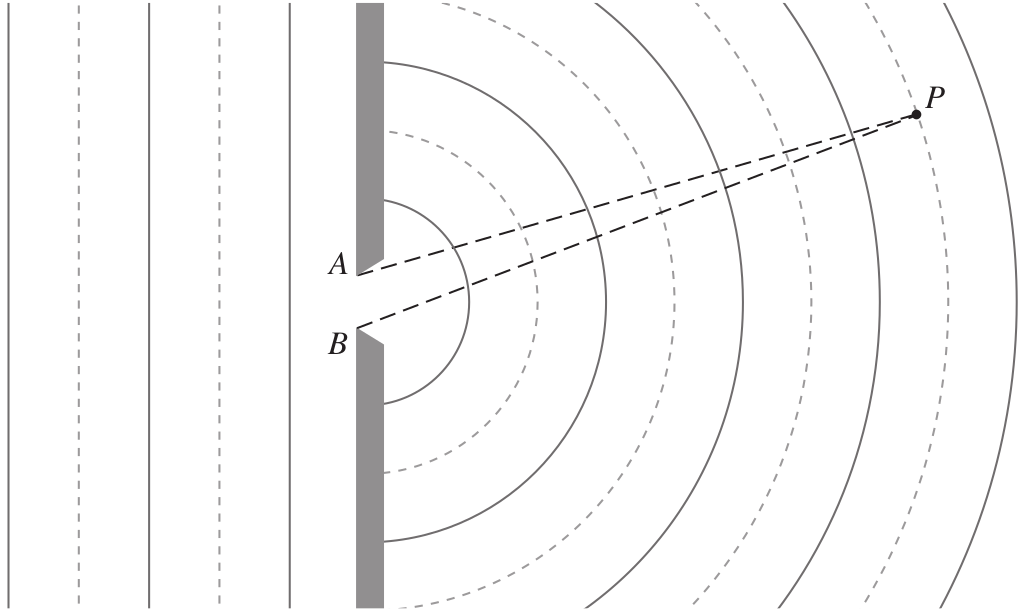
\includegraphics[width= 0.9 \linewidth]{1_INTRO/direcciones.png}
	\caption{Propagación de la onda.}
	\label{fig:rectang}
\end{minipage}
\end{figure}
\begin{figure}[hbt!]
	\addfontfeature{LetterSpace = -5}
	\begin{minipage}{0.4\linewidth}
	\centering
	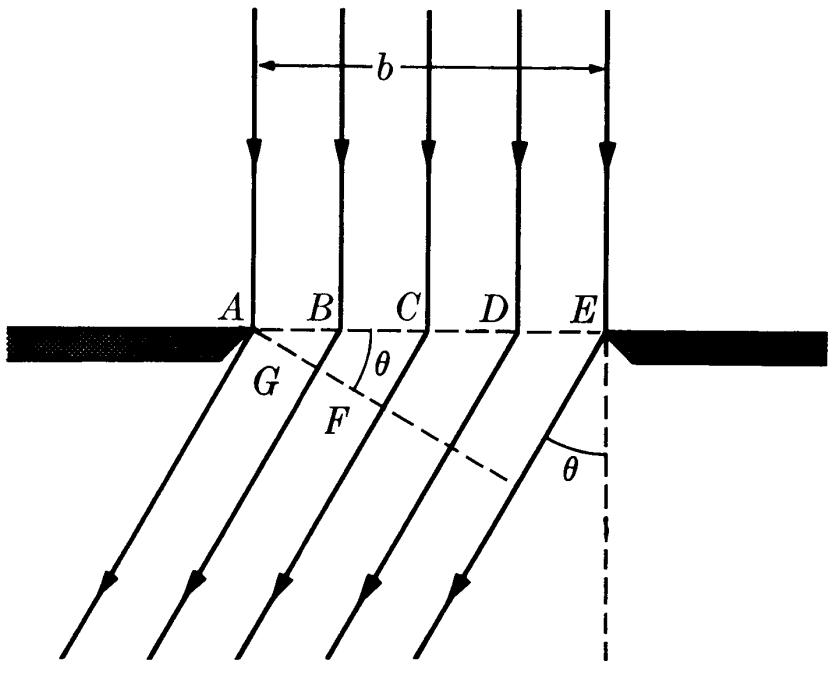
\includegraphics[width= \linewidth]{1_INTRO/seno.png}
	\caption{Difracción de la onda en la dirección del ángulo \(\theta\).}
	\label{fig:seno}
	\end{minipage}\hspace{5mm}
	\begin{minipage}{0.6\linewidth}
		Entonces, las ondas que atraviesen la rendija alcanzarán un máximo en la onda, en aquellos ángulos \(\theta\), tal que las continuaciones de los rayos coincidan con los máximos antes de golpear la rendija, Como lo indica la Figura \ref{fig:seno} (obtenida de \micita{alonso_finn_1}).
		Es decir, si \(d\) es el tamaño de la rendija, \(\lambda\) la longitud de onda, y \(\theta\) el ángulo de desviación, tendremos:
		\begin{equation}
			d \sin \theta = m \lambda , \hspace{1cm} m \in \mathds{Z}.
			\label{eq:posicion_angular}
		\end{equation}
	\end{minipage}
\end{figure}
\begin{figure}[hbtp!]
	\addfontfeature{LetterSpace = -5}
	\begin{minipage}{0.5\linewidth}
		Además, notamos que si el ángulo \(\theta\) es suficientemente pequeño, \(y\) es la distancia del máximo central al \(m-\)ésimo máximo de la ec. (\ref{eq:posicion_angular}), y \(D\) es la separación de una pantalla con la rendija, entonces se tendrá \(\sin \theta = \tan \theta\), y \vspace{-3mm}
		\begin{equation}
			\tan \theta = \dfrac{y}{D}.
			\label{eq:distan_rendija}
		\end{equation}
		Así, como lo indica la Figura \ref{fig:constructiva}. Combinando (\ref{eq:posicion_angular}) y (\ref{eq:distan_rendija}), obtenemos que
		\begin{equation}
			y = \dfrac{m \lambda D}{d} , \hspace{1cm} m \in \mathds{Z} .
			\label{eq:altura}
		\end{equation}
	\end{minipage}\hspace{5mm}
	\begin{minipage}{0.5\linewidth}
		\centering
		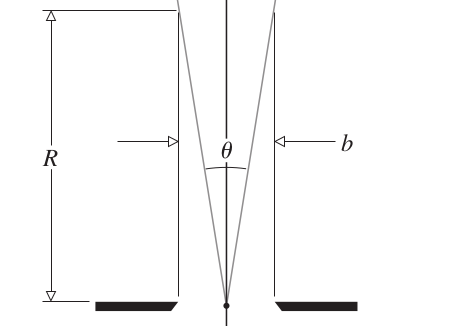
\includegraphics[width= \linewidth, height = 8.5cm]{1_INTRO/distancia}
		\caption{Tamaño de la difracción constructiva.}
		\label{fig:constructiva}
	\end{minipage}
\end{figure}
% )))

\subsection{--- Difracción de Doble Rendija ---} % (((
\label{sub:difraccion_dos}
Ahora, consideremos dos rendijas, ambas de tamaño \(a\), separadas a una distancia \(d\), como lo indica la Figura \ref{fig:exp_young}, al cual se le conoce como \textbf{Experimento de Young}.
\begin{figure}[hbt!]
	\centering
	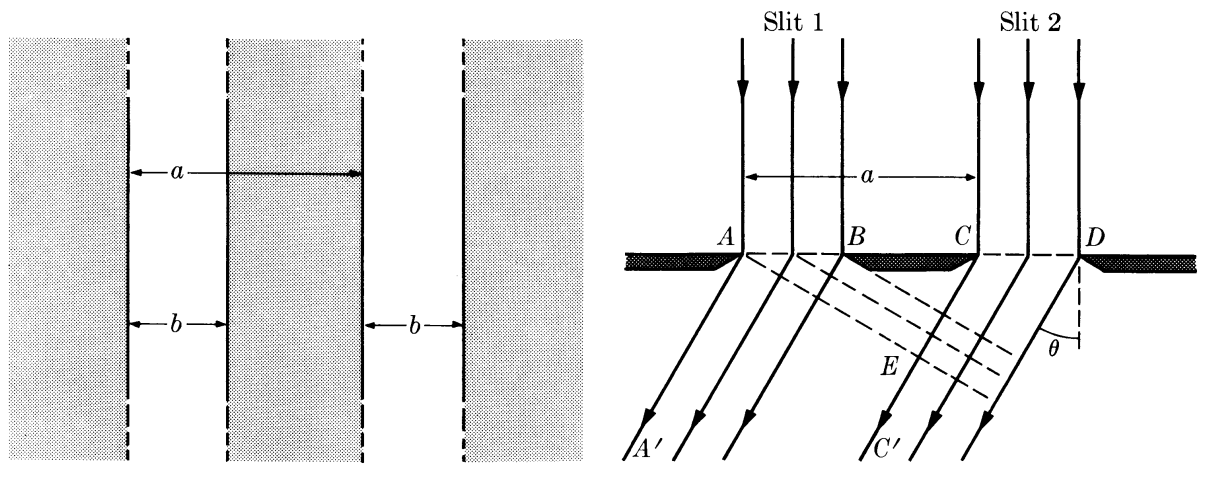
\includegraphics[width= \linewidth]{1_INTRO/dos_rendijas.png}
	\caption{Experimento de Young.}
	\label{fig:exp_young}
\end{figure}\\
Notamos que la diferencia de fase entre ambas ondas es de
\[
	\alpha = \dfrac{2 \pi}{\lambda} CE = \dfrac{2 \pi d \sin \theta}{\lambda}.
\]
\begin{figure}[hbtp!]
	\addfontfeature{LetterSpace = -5}
	\begin{minipage}{0.5\linewidth}
	Notamos que, para la difracción de Faunhofer, se tiene la situación de la Figura \ref{fig:radios}. \\[2mm]
	Entonces, \(r \approx R - y \sin \theta\), y por cada rendija se tiene que 
		\[
			F(y) = \sin (wt- kr) = \sin (wt-k(R - y \sin \theta))
		\]
		Y también, para cada rendija tendremos la siguiente expresión para el campo eléctrico,
		\[
			E = C \dis\int _{y_{min}} ^{y_{max}} F(y) dy.
		\]
		Indicando que, en nuestro caso con dos rendijas, y con las longitudes de la Figura \ref{fig:exp_young}, obtendremos que
	\end{minipage}\hspace{5mm}
	\begin{minipage}{0.5\linewidth}
	\centering
	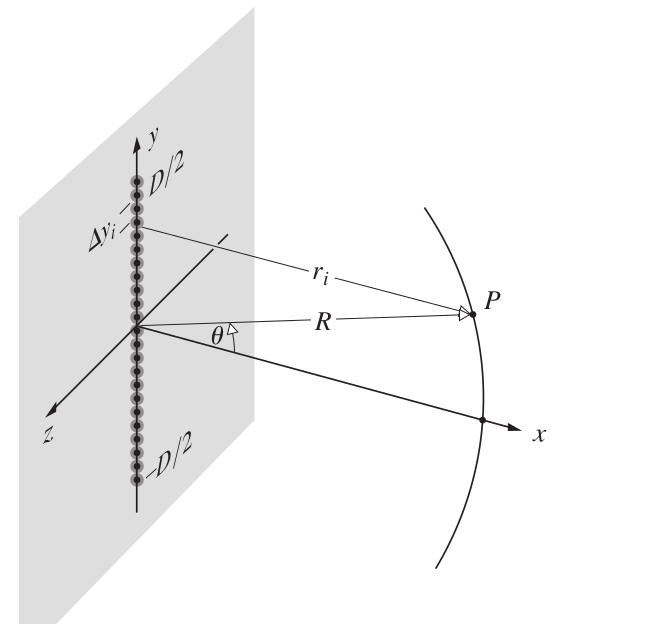
\includegraphics[width= 0.8 \linewidth]{1_INTRO/fran}
	\caption{Radios hacia la rendija.}
	\label{fig:radios}
	\end{minipage}
\end{figure}
\begin{equation}
	\begin{array}{rcl}
		E & = & C \dis\int _{-a/2} ^{a/2} F(y) dy + C \dis\int _{d-a/2} ^{d+a/2} F(y) dy\\[5mm]
		& = & bC \bigg(\dfrac{\sin \beta}{\beta}\bigg) \big(\sin (wt-kR) + \sin (wt-kR + 2\alpha)\big)
	\end{array}
	\label{eq:campo_electrico}
\end{equation}
donde \(\beta = \dfrac{kb}{2} \sin \theta\), y \(\alpha = \dfrac{ka}{2} \sin \theta\). La gráfica de ésta función se deja indicada en la Figura \ref{fig:grafica}. 
\begin{figure}[hbt!]
	\centering
	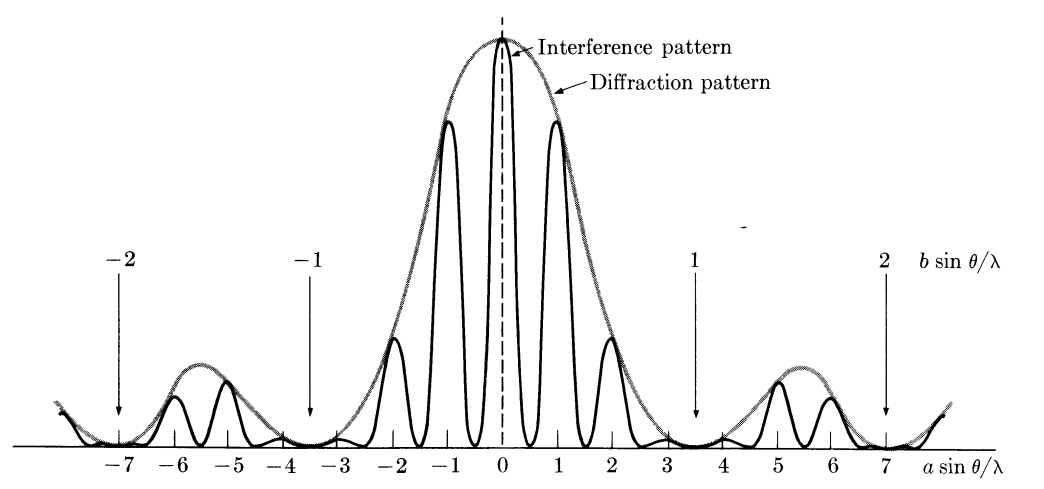
\includegraphics[width= 0.7 \linewidth]{1_INTRO/grafica}
	\caption{Gráfica de la función (4).}
	\label{fig:grafica}
\end{figure}\\
Además, se tiene la siguiente irradiancia.
\begin{equation}
	I= \langle E \rangle ^2/2 = 4I_0 \bigg(\dfrac{\sin ^2 \beta}{\beta ^2}\bigg) \cos ^2\alpha
	\label{eq:irradiancia}
\end{equation}
y se le llama irradiancia ``normalizada'' a la función \(I/(4I_0)\).
% )))

\subsection{--- Métodos de Análisis Experimental ---} % (((
\label{sub:metodos_analisis}
El propósito del sistema físico del experimento de Young en ésta práctica es el de presenciar, primero, los patrones de difracción por el tamaño de las rendijas, y segundo, observar el patrón de interferencia generado por la simultaneidad de las dos rendijas del experimento.
Con éste objetivo, se pudo controlar el tamaño y separación de las rendijas para cotejar los valores obtenidos de forma empírica con los teóricos.
Por tanto, se esperan obtener los máximos de forma similar a una curva de nivel de la función (\ref{eq:campo_electrico}) expresada en la Figura \ref{fig:grafica}.
% )))

% )))

\section{METODOLOGÍA.} % (((
\begin{enumerate}[noitemsep]
	\item La incertidumbre del Vernier es de $ 0.01cm/2=0.005 cm $
	\item La incertidumbre de la cinta métrica es de $ 0.1cm/2=0.05 cm $
\end{enumerate}
La Figura \ref{fig:conf_inicial} muestra la configuración inicial para el dispositivo experimental usado.
Se posiciona mediante un banco óptico el láser, el disco de rendijas y la pantalla cuadriculada en ese orden respectivamente, de tal manera que, al encender el láser, éste pasará por alguna de las configuraciones para el disco óptico mostrando en la pantalla el patrón de interferencia generado.
\begin{figure}[hbtp!]
	\centering
	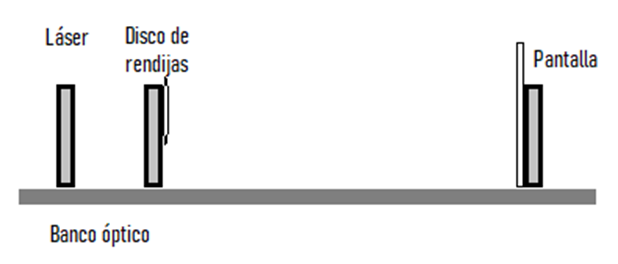
\includegraphics[width= 0.7 \linewidth]{2_METODO/image}
	\caption{Configuración inicia del experimento.}
	\label{fig:conf_inicial}
\end{figure}\\
Para poder obtener el patrón fue necesario ajustar la distancia entre los 3 componentes y alinear el sistema tal que el haz láser lograse incidir en la rendija, con lo cual, se procedió a encender el láser ajustando la alineación del patrón para que coincidiese con la cuadrícula de la pantalla, y así poder realizar 2 mediciones a cada una de las 4 distintas configuraciones del disco de rendijas usadas, las cuales fueron la distancia del máximo 0 al máximo 2 y del máximo 0 al máximo 4.
\begin{figure}[hbtp!]
	\addfontfeature{LetterSpace = -5}
	\begin{minipage}{0.3 \linewidth}
		\centering
		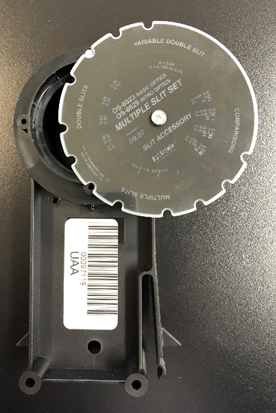
\includegraphics[height = 6cm]{2_METODO/image_2}
		\caption{Láser usado en el experimento}
		\label{fig:laser}
	\end{minipage} \hspace{4mm}
	\begin{minipage}{0.3 \linewidth}
		\centering
		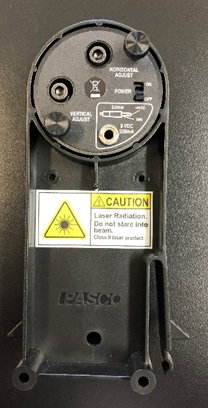
\includegraphics[height = 6cm]{2_METODO/image_3}
		\caption{Disco con sus diferentes rendijas.}
		\label{fig:disco}
	\end{minipage} \hspace{4mm}
	\begin{minipage}{0.3 \linewidth}
		\centering
		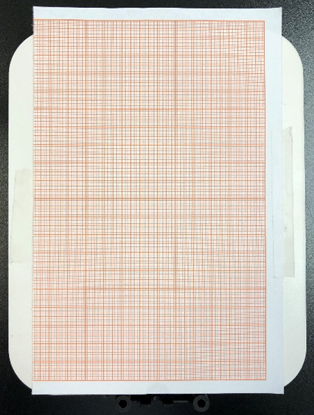
\includegraphics[height = 6cm]{2_METODO/image_4}
		\caption{Pantalla cuadriculada.}
		\label{fig:pantalla}
	\end{minipage}
\end{figure}
\newpage
Decidir el máximo 0 fue tarea de encasillar los máximos entre los de menor intensidad dentro de la región en la que se presentaba mayor saturación, contándolos y obteniendo el central como se muestra en la Figura \ref{fig:patron}.
\begin{figure}[hbtp!]
	\addfontfeature{LetterSpace = -5}
	\centering
	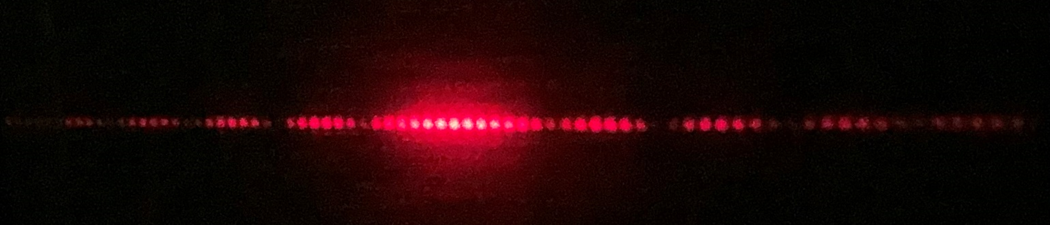
\includegraphics[width= 0.7 \linewidth]{2_METODO/image_5}
	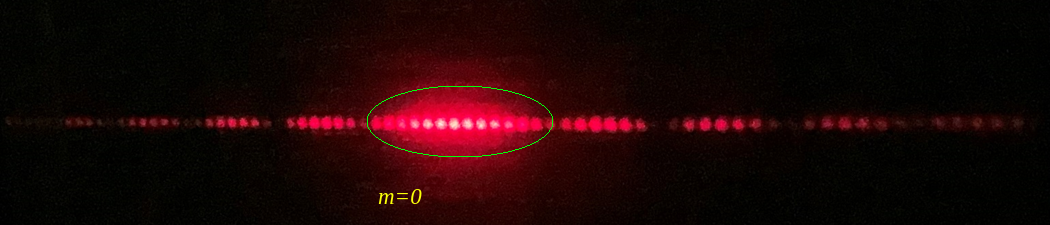
\includegraphics[width= 0.7 \linewidth]{2_METODO/image_6_1}
	\caption{Fotografía para el patrón formado por la rendija de tipo \(a= 0.04mm\), y \(d=0.25mm\). Se encierra (en verde) la región central que presenta la mayor saturación y que está delimitada por los máximos de menor intensidad respectivos. Se marca \(m=0\) en amarillo.}
	\label{fig:patron}
\end{figure}
% )))

\section{RESULTADOS.} % (((

\subsection{--- Comparación Máximos Teóricos y Experimentales ---} % (((
\label{sub:comparacion}
	 Durante el experimento, se tenían los siguientes datos ``fijos$"$:
	 \begin{itemize}
	 	\item La distancia $ D $ entre la doble rendija y la pantalla era $ D=(90\pm 0.05) cm$
	 	\item La longitud de la onda del láser empleado era de $ \lambda=650 nm=6.5\times 10^{-5}cm $
	 \end{itemize}
	 \newpage
 	Luego, para dos máximos de interferencia elegidos $ (m_1, m_2) $ en la pantalla, y considerando un ancho de rendija $ a $ separadas una distancia $ d $, la distancia $ y $ entre tales máximos elegidos se muestran en la siguiente tabla \ref{tab:distancias}
 	\begin{table}[!htb]
 		\centering
 		\caption{Distancias entre máximos observados}
 		\begin{tabular}{|c|c|c|}
 			\hline
			\backslashbox{$ a, d $ (\(mm\))}{$ (m_1,m_2) $}& $ (0,2) $ & $ (0,4) $ \\
 			\hline
 			$ a=0.04 $ & \multirow{2}{*}{$ (0.395\pm 0.005) cm $} & \multirow{2}{*}{$ (0.845\pm 0.005) cm $} \\ 		
 			$ d=0.25 $ &  & \\ 
 			\hline
 			$ a=0.08 $& \multirow{2}{*}{$ (0.380\pm 0.005) cm $} & \multirow{2}{*}{$ (0.870\pm 0.005) cm $} \\
 			$ d=0.25 $&  &  \\
 			\hline
 			$ a=0.04 $          & \multirow{2}{*}{$ (0.215\pm 0.005) cm $} & \multirow{2}{*}{$ (0.430\pm 0.005) cm $} \\ 		
 			$ d=0.5\phantom{0} $&  &  \\	
 			\hline
 			$ a=0.08 $           & \multirow{2}{*}{$ (0.180 \pm 0.005) cm $} & \multirow{2}{*}{$ (0.420 \pm 0.005) cm $} \\
 			$ d=0.5\phantom{0} $ &  &  \\
 			\hline
 		\end{tabular}
 		\label{tab:distancias}
 	\end{table}\\
		Haciendo uso de la ecuación (\ref{eq:altura}), para los mismos valores anteriores se tienen las siguientes distancias teóricas (tabla \ref{tab:disteo}).
 	\begin{table}[hbtp!]
 		\centering
 		\caption{Distancias teóricas para los máximos}
 		\begin{tabular}{|c|c|c|}
 			\hline
			$ d $ (\(mm\)) & \multicolumn{2}{c|}{$ y_m $ (\(cm\))}  \\
 			\hline
 			0.25 & $ y_2=0.4680\pm 0.0002 $ & $ y_4=0.9360\pm0.0005 $ \\
 			\hline
 			0.5 & $ y_2=0.2340\pm 0.0001 $ & $ y_4=0.4680\pm0.0002 $  \\
 			\hline
 		\end{tabular}
 		\label{tab:disteo}
 	\end{table}\\
 	A continuación, en la tabla \ref{tab:errores} se calculan los errores absolutos y relativos de las mediciones obtenidas
 	\begin{table}[!htb]
 		\centering
 		\caption{Errores absolutos y relativos}
 		\begin{tabular}{|c|c|c|c|c|}
 			\hline
			$ a, d $ (\(mm\)) & $ y_m $ observado (\(cm\)) & $ y_m $ teórico (\(cm\)) & Error absoluto (\(cm\)) & Error relativo (\textsc{\%})  \\
 			\hline
 			$ a=0.04 $          & $y_2=0.395\pm 0.005 $ & $y_2=0.4680\pm0.0002 $ & $ 0.073 $ & $ 15.59 $ \\ \cline{2-5}
 			$ d=0.25 $          & $y_4=0.845\pm 0.005 $ & $y_4=0.9360\pm0.0005 $ & $ 0.091 $ & $ \phantom{0}9.72 $ \\ \hline
 			$ a=0.08 $          & $y_2=0.380\pm 0.005 $ & $y_2=0.4680\pm0.0002 $ & $ 0.088 $ & $ 18.80 $ \\ \cline{2-5}
 			$ d=0.25 $          & $y_4=0.870\pm 0.005 $ & $y_4=0.9360\pm0.0005 $ & $ 0.066 $ & $ \phantom{0}7.05 $ \\ \hline
 			$ a=0.04 $          & $y_2=0.215\pm 0.005 $ & $y_2=0.2340\pm0.0001 $ & $ 0.019 $ & $ \phantom{0}8.11 $ \\ \cline{2-5}
 			$ d=0.5\phantom{0} $& $y_4=0.430\pm 0.005 $ & $y_4=0.4680\pm0.0002 $ & $ 0.038 $ & $ \phantom{0}8.11 $ \\ \hline
 			$ a=0.08 $          & $y_2=0.180\pm 0.005 $ & $y_2=0.2340\pm0.0001 $ & $ 0.054 $ & $ 23.07 $ \\ \cline{2-5}
 			$ d=0.5\phantom{0} $& $y_4=0.420\pm 0.005 $ & $y_4=0.4680\pm0.0002 $ & $ 0.048 $ & $ 10.25 $ \\ \hline
 		\end{tabular} 
 		\label{tab:errores}
 	\end{table}\\
	En las Figuras 12--23 de las siguientes secciones se establece la comparativa gráfica en la función de obtenida experimentalmente, contra la teórica con los parámetros dados.
% )))

	\newpage

	\subsection{--- \(a=0.04mm\), \(d=0.25mm\) ---} % (((
	\label{sub:a_bajo_d_bajo}
	\begin{figure}[htbp!]
		\centering
		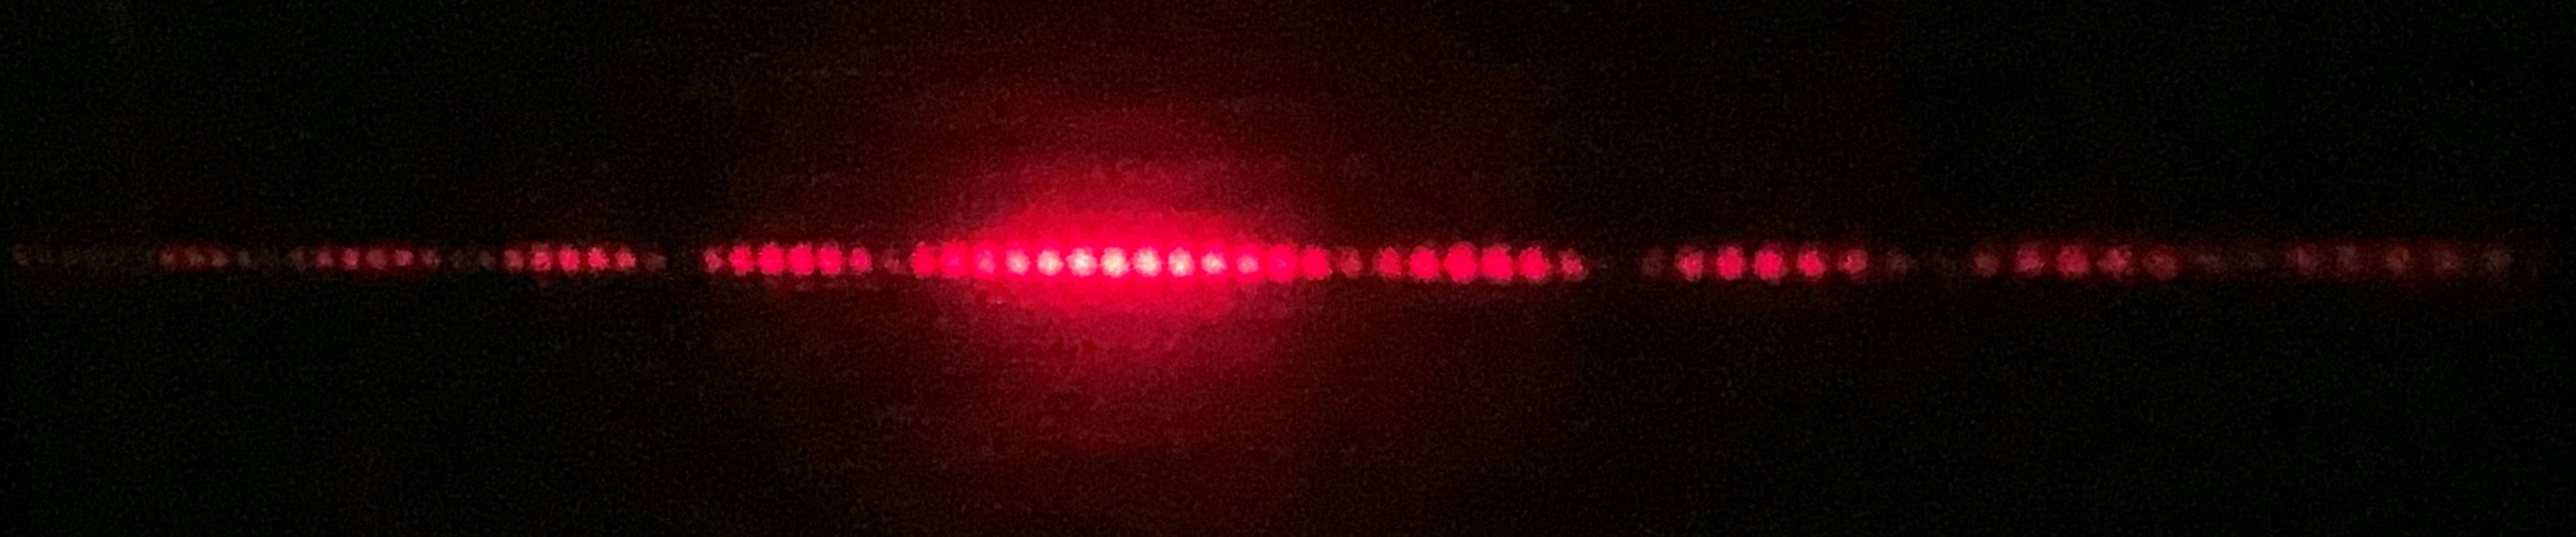
\includegraphics[width=0.7\textwidth]{3_RESUL/04_y_25.jpg}
		\caption{Foto de la rendija}
		\label{fig:A1}
		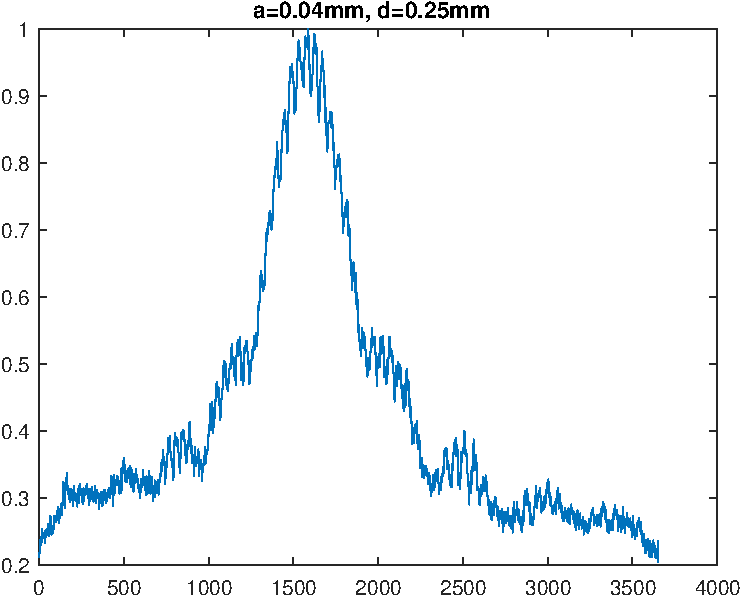
\includegraphics[width=0.7\linewidth,height=8cm]{3_RESUL/04_y_25.pdf}
		\caption{Patrón de irradiancia experimental}
		\label{fig:A2}
		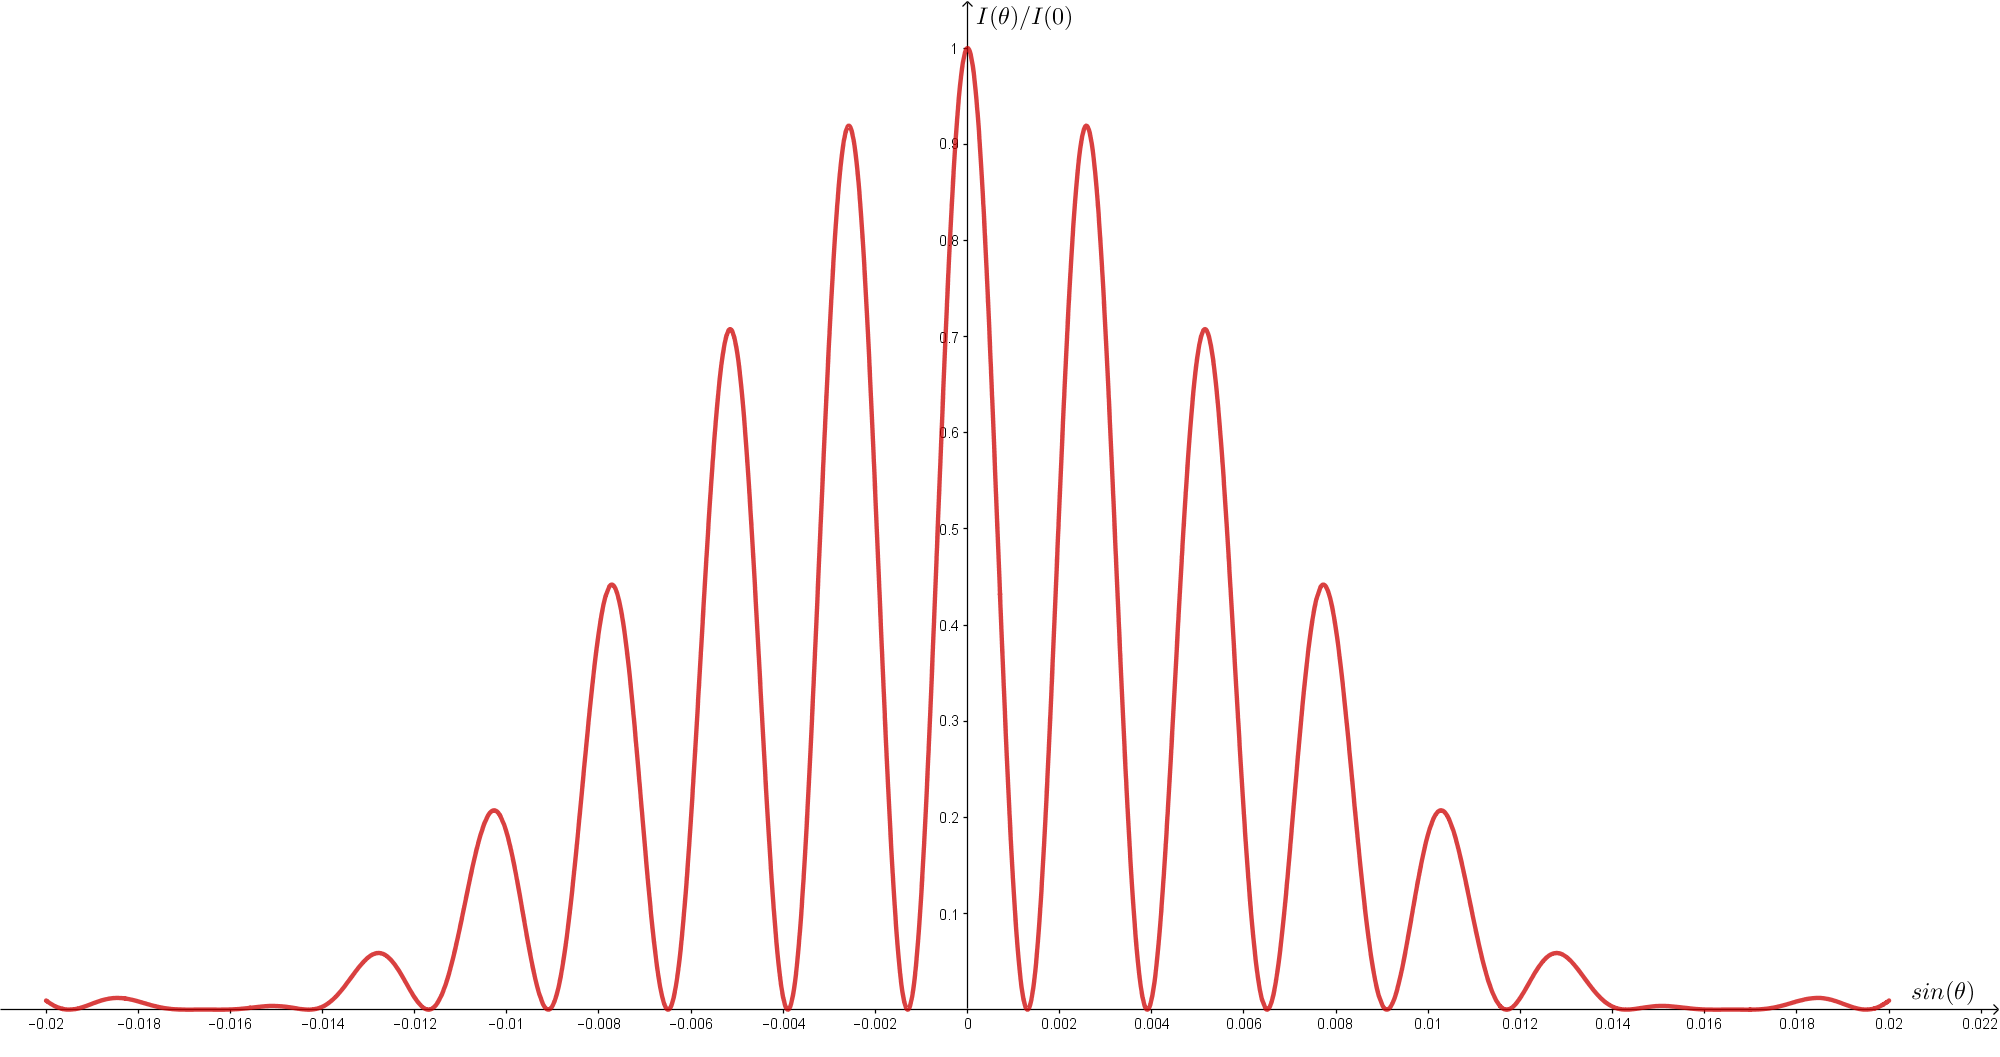
\includegraphics[width=0.7\linewidth,height=8cm]{3_RESUL/Irradiancia 1.png}
		\caption{Patrón de irradiancia teórico}
		\label{fig:A3}
		% \caption{Patrones de irradiancia para la rendija indicada}
		% \label{fig:P1}
	\end{figure}
	% )))

	\newpage
	\subsection{--- \(a=0.08mm\), \(d=0.25mm\) ---} % (((
	\label{sub:a_alto_d_bajo}
	\begin{figure}[htbp!]
		\centering
		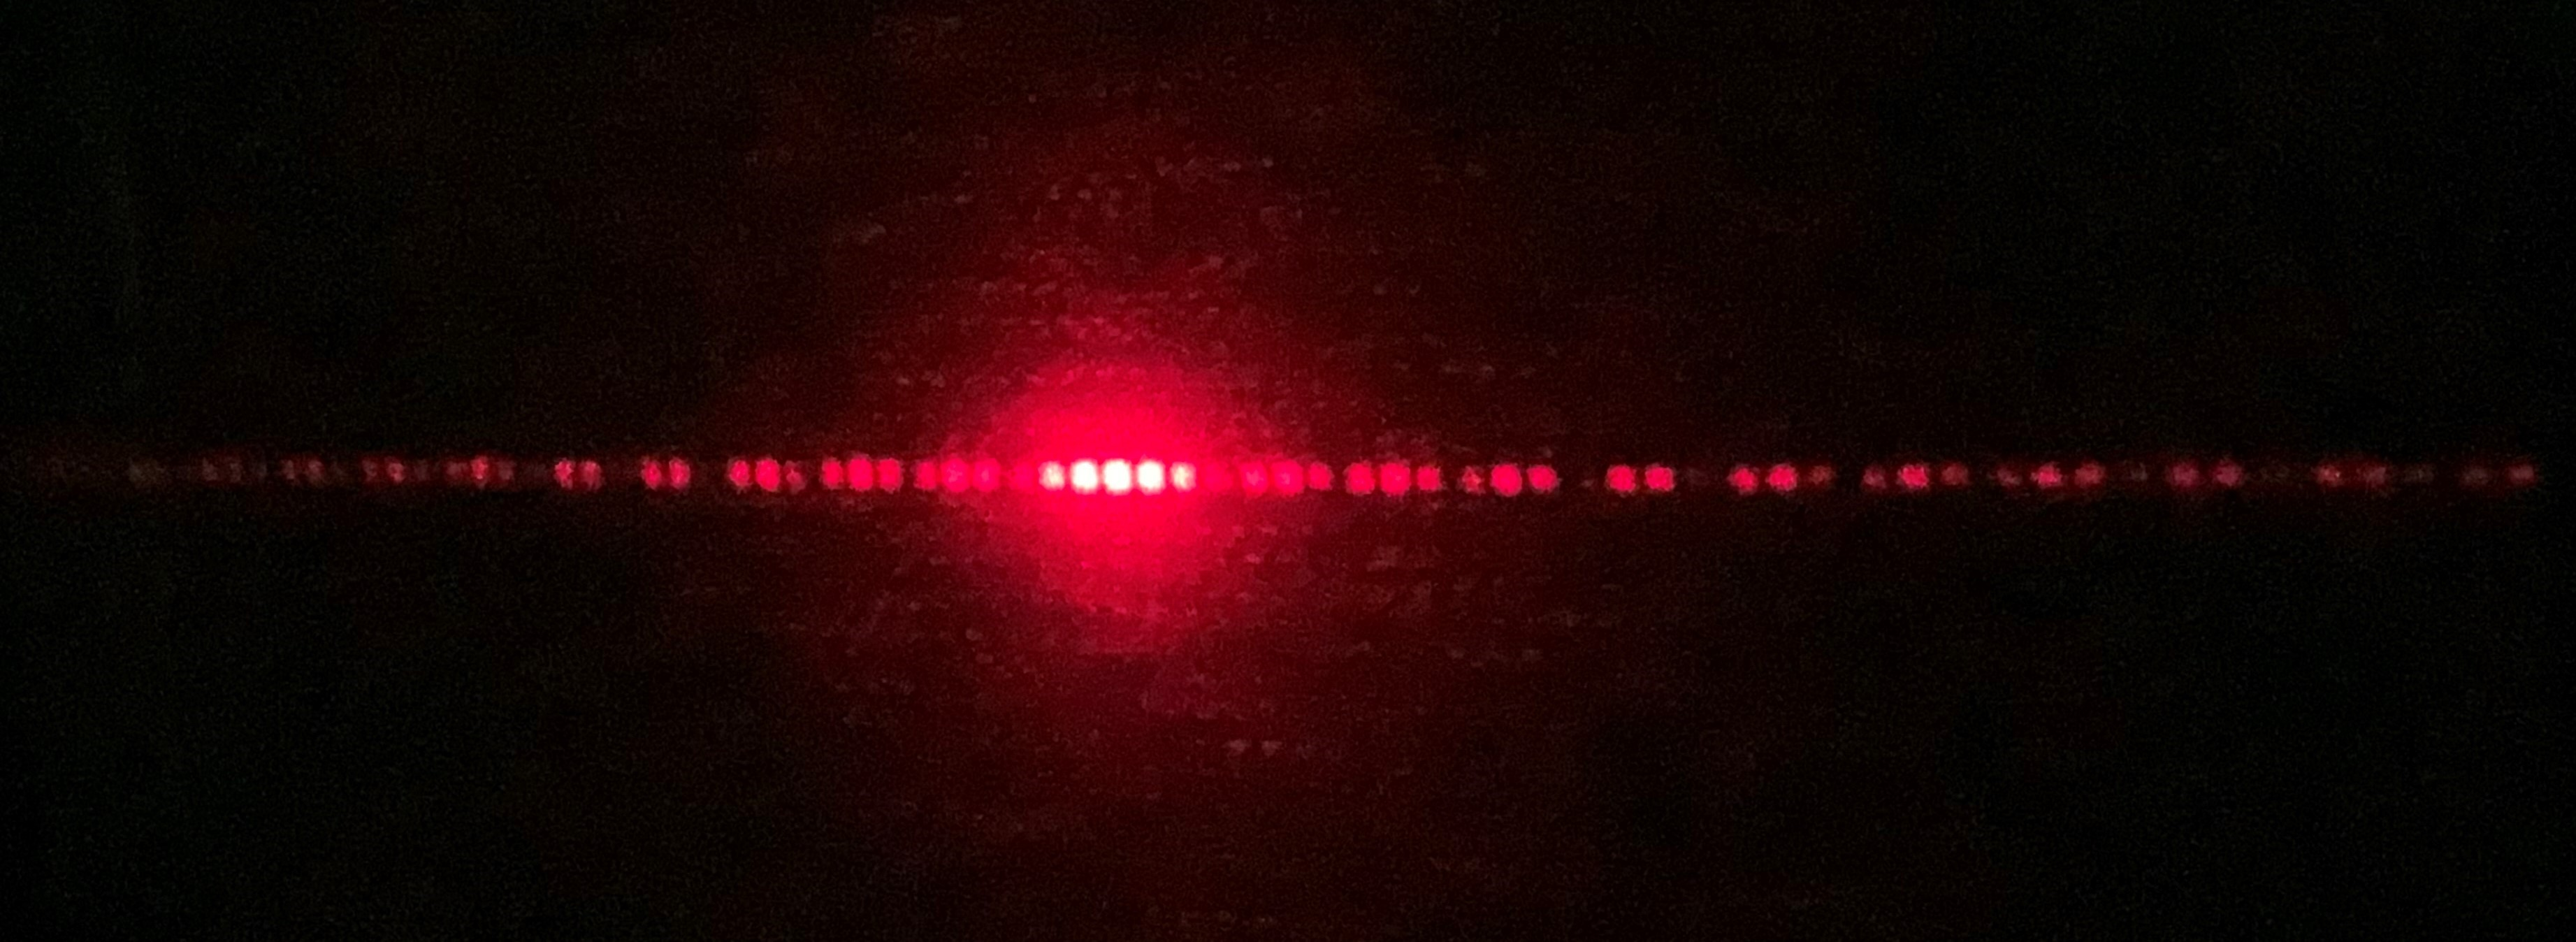
\includegraphics[width=0.7\textwidth, height=3cm]{3_RESUL/08_y_25.jpg}
		\caption{Foto de la rendija}
		\label{fig:A4}
		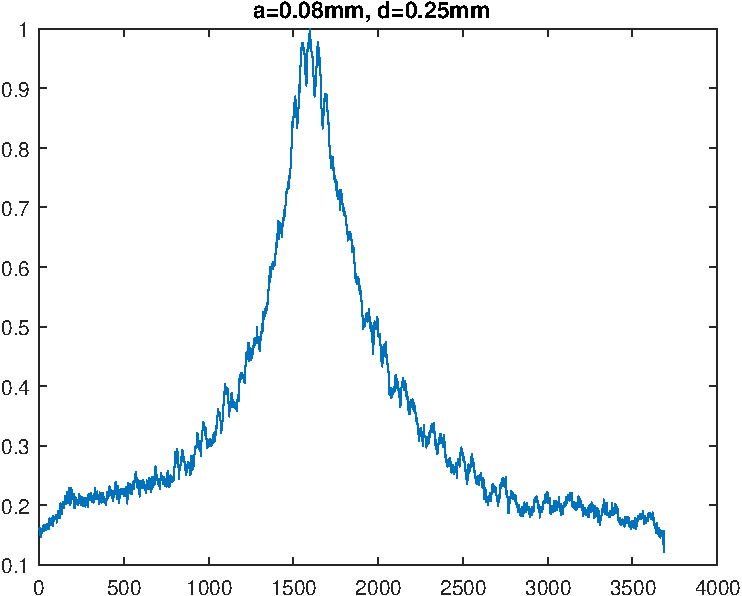
\includegraphics[width=0.7\linewidth,height=7cm]{3_RESUL/08_y_25.pdf}
		\caption{Patrón de irradiancia experimental}
		\label{fig:A5}
		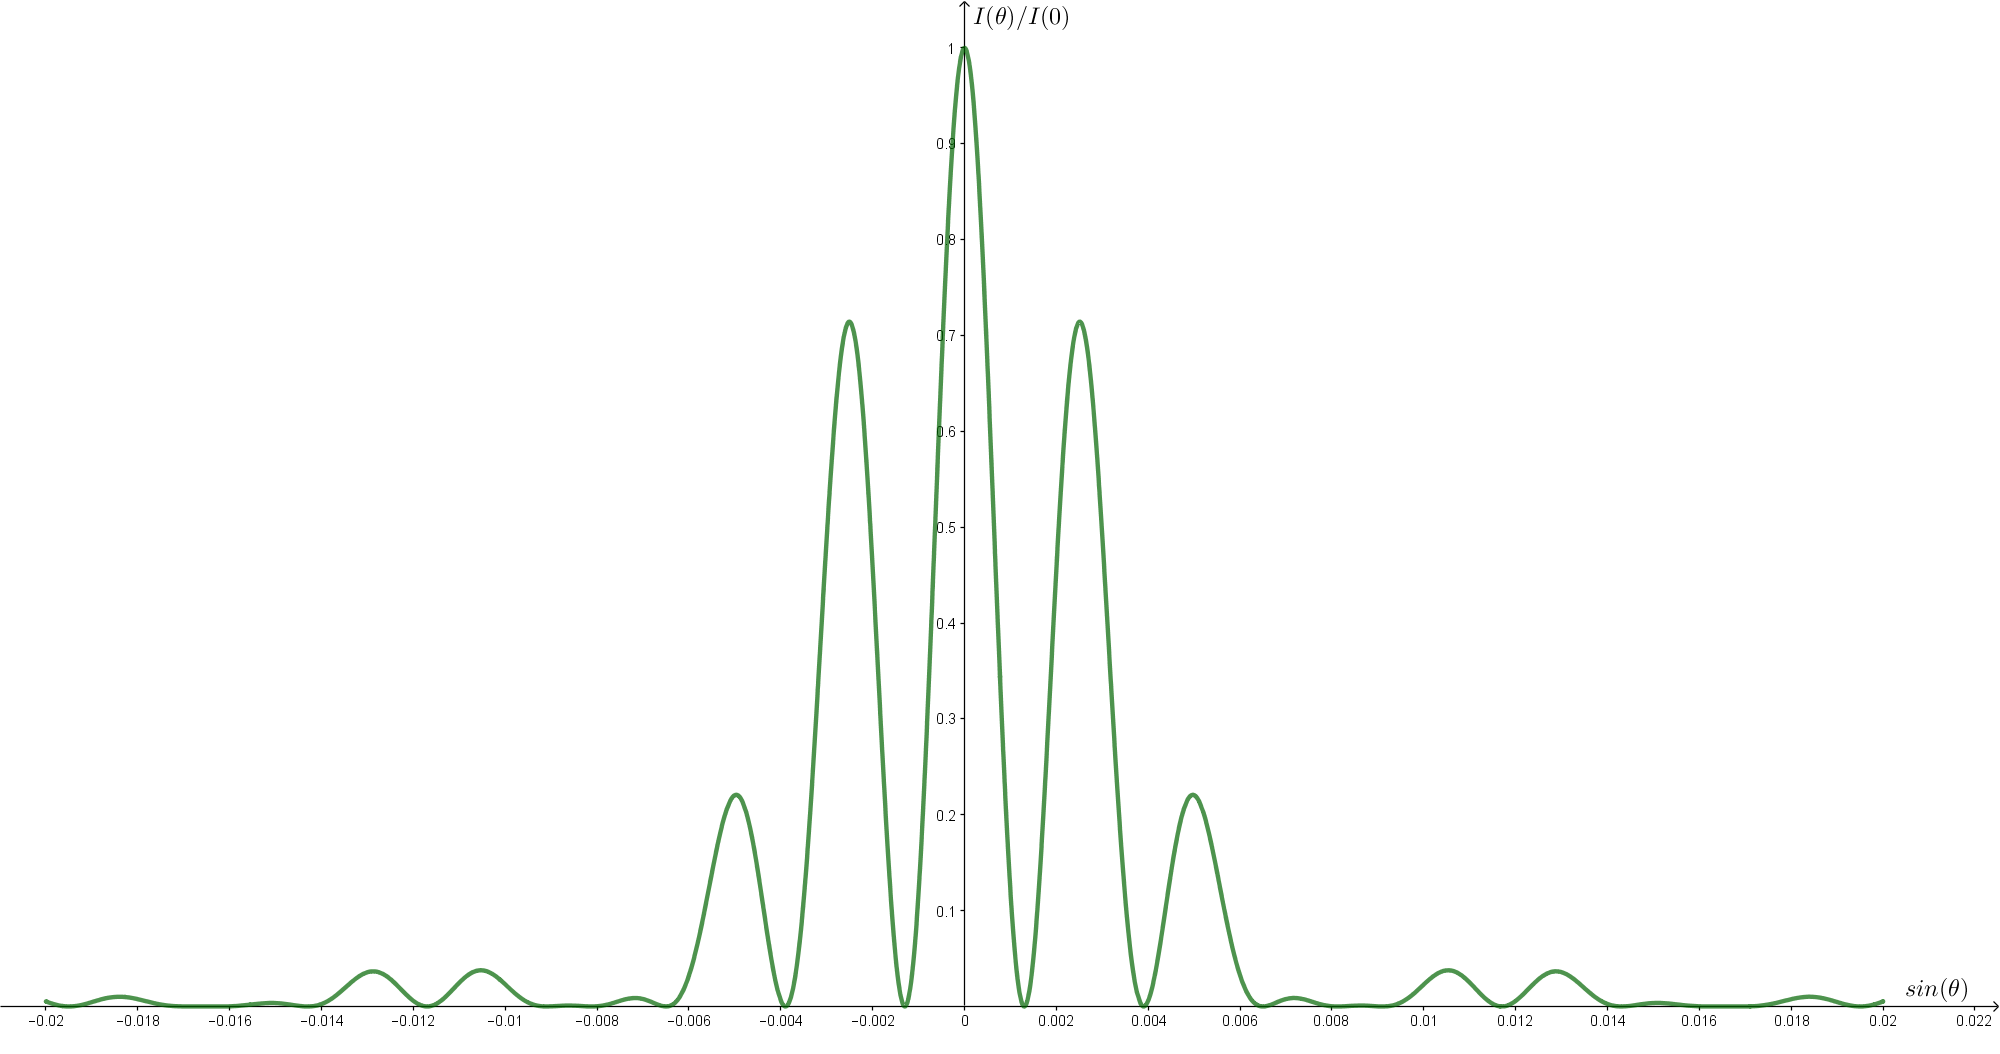
\includegraphics[width=0.7\linewidth,height=7.5cm]{3_RESUL/Irradiancia 2.png}
		\caption{Patrón de irradiancia teórico}
		\label{fig:A6}
		% \caption{Patrones de irradiancia para la rendija indicada}
		% \label{fig:P2}
	\end{figure}
	% )))

	\newpage
	\subsection{--- \(a=0.04mm\), \(d=0.5mm\) ---} % (((
	\label{sub:a_bajo_d_alto}
	\begin{figure}[htbp!]
		\centering
		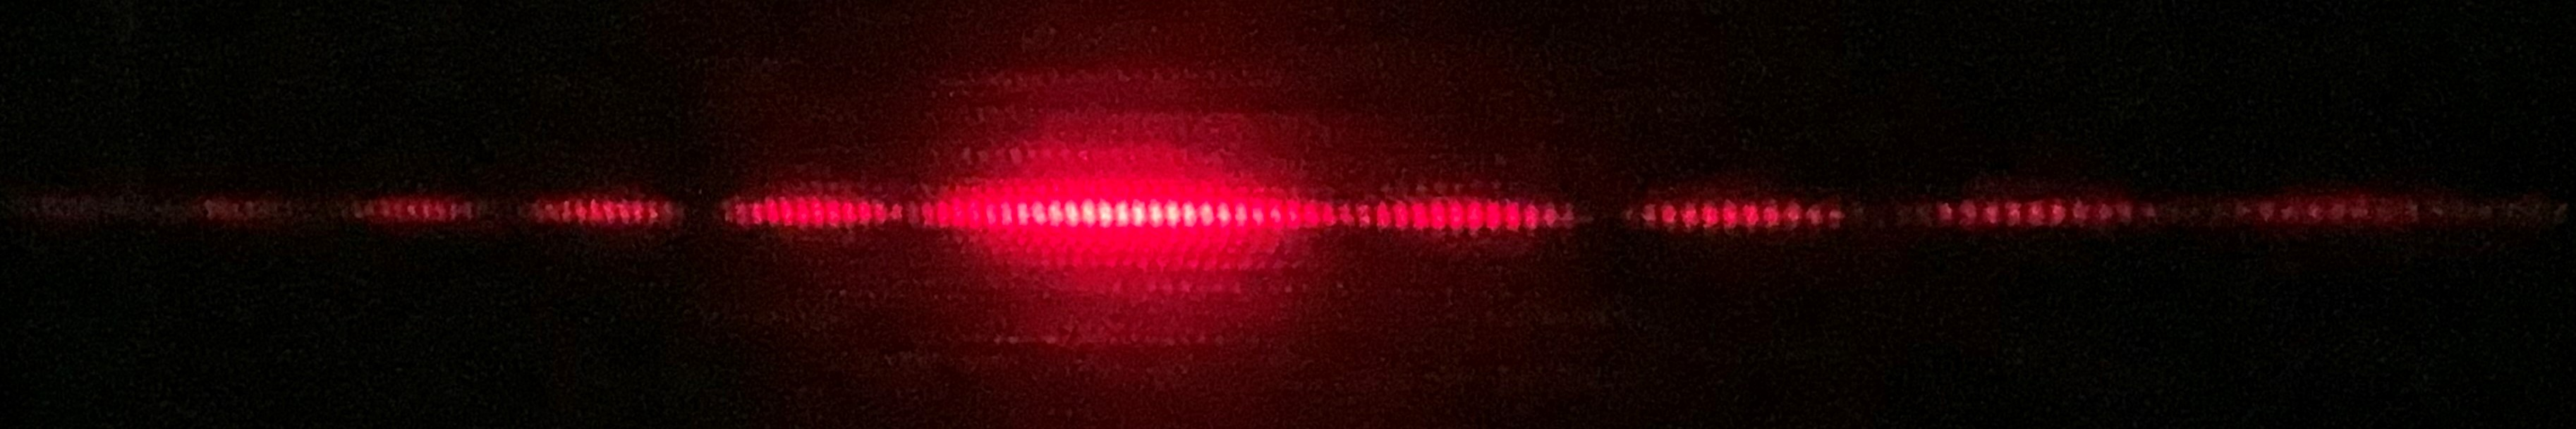
\includegraphics[width=0.7\textwidth]{3_RESUL/04_y_5.jpg}
		\caption{Foto de la rendija}
		\label{fig:A7}
		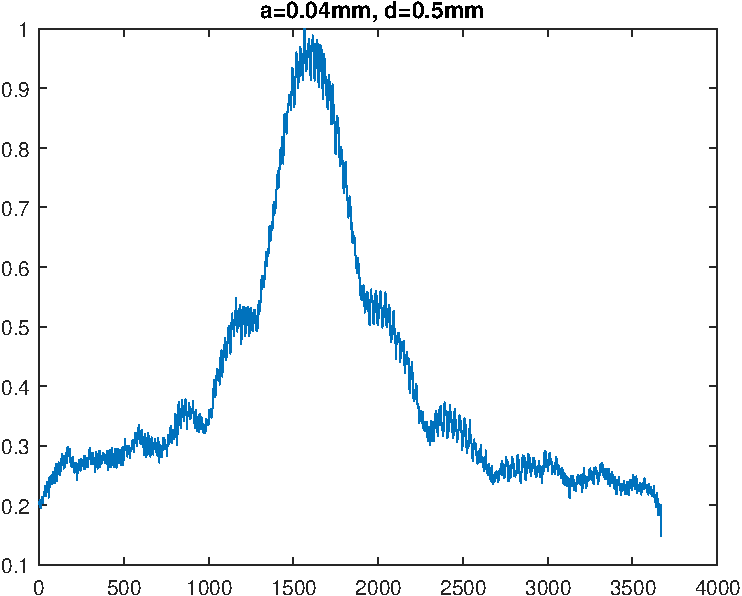
\includegraphics[width=0.7\linewidth,height=8cm]{3_RESUL/04_y_5.pdf}
		\caption{Patrón de irradiancia experimental}
		\label{fig:A8}
		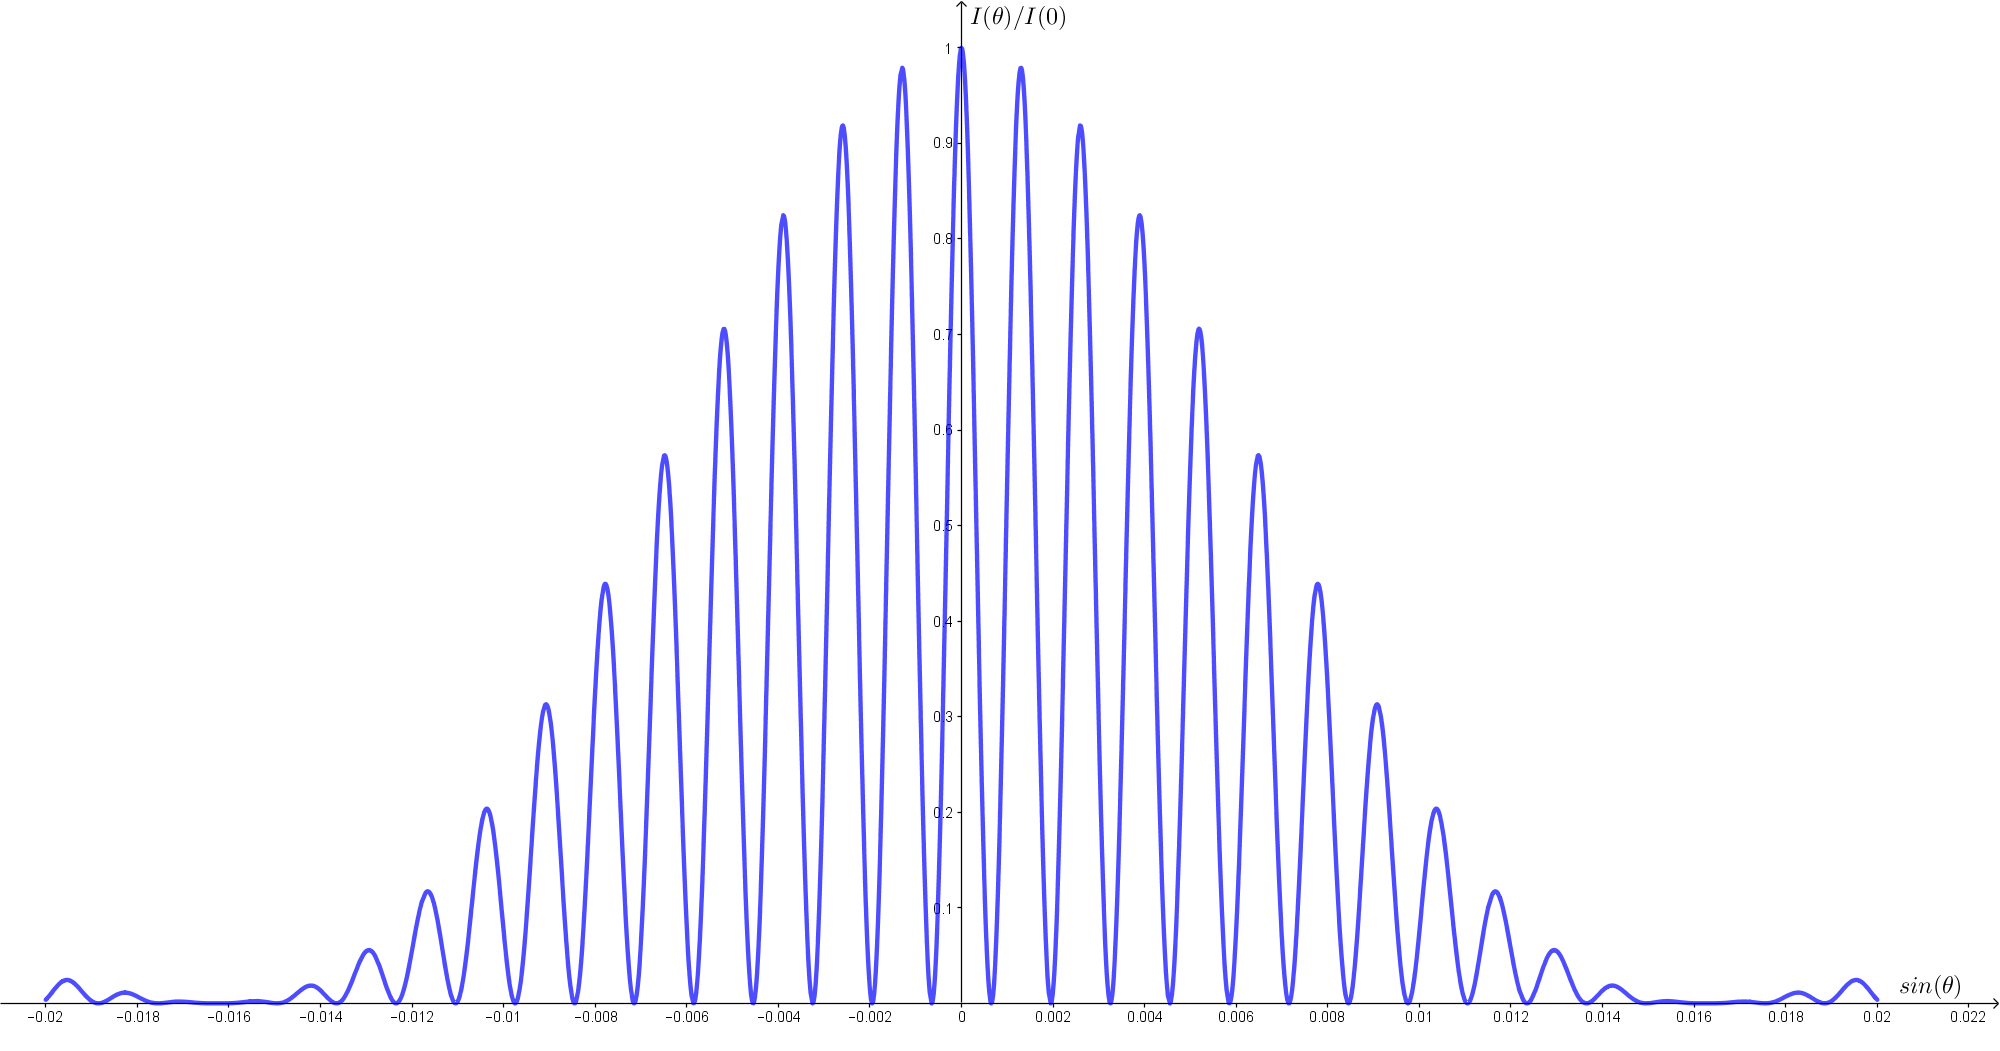
\includegraphics[width=0.7\linewidth,height=8cm]{3_RESUL/Irradiancia 3.png}
		\caption{Patrón de irradiancia teórico}
		\label{fig:A9}
		% \caption{Patrones de irradiancia para la rendija indicada}
		% \label{fig:P3}
	\end{figure}
	% )))

	\newpage
	\subsection{--- \(a=0.08mm\), \(d=0.5mm\) ---} % (((
	\label{sub:a_alto_d_alto}
	\begin{figure}[htbp!]
		\centering
		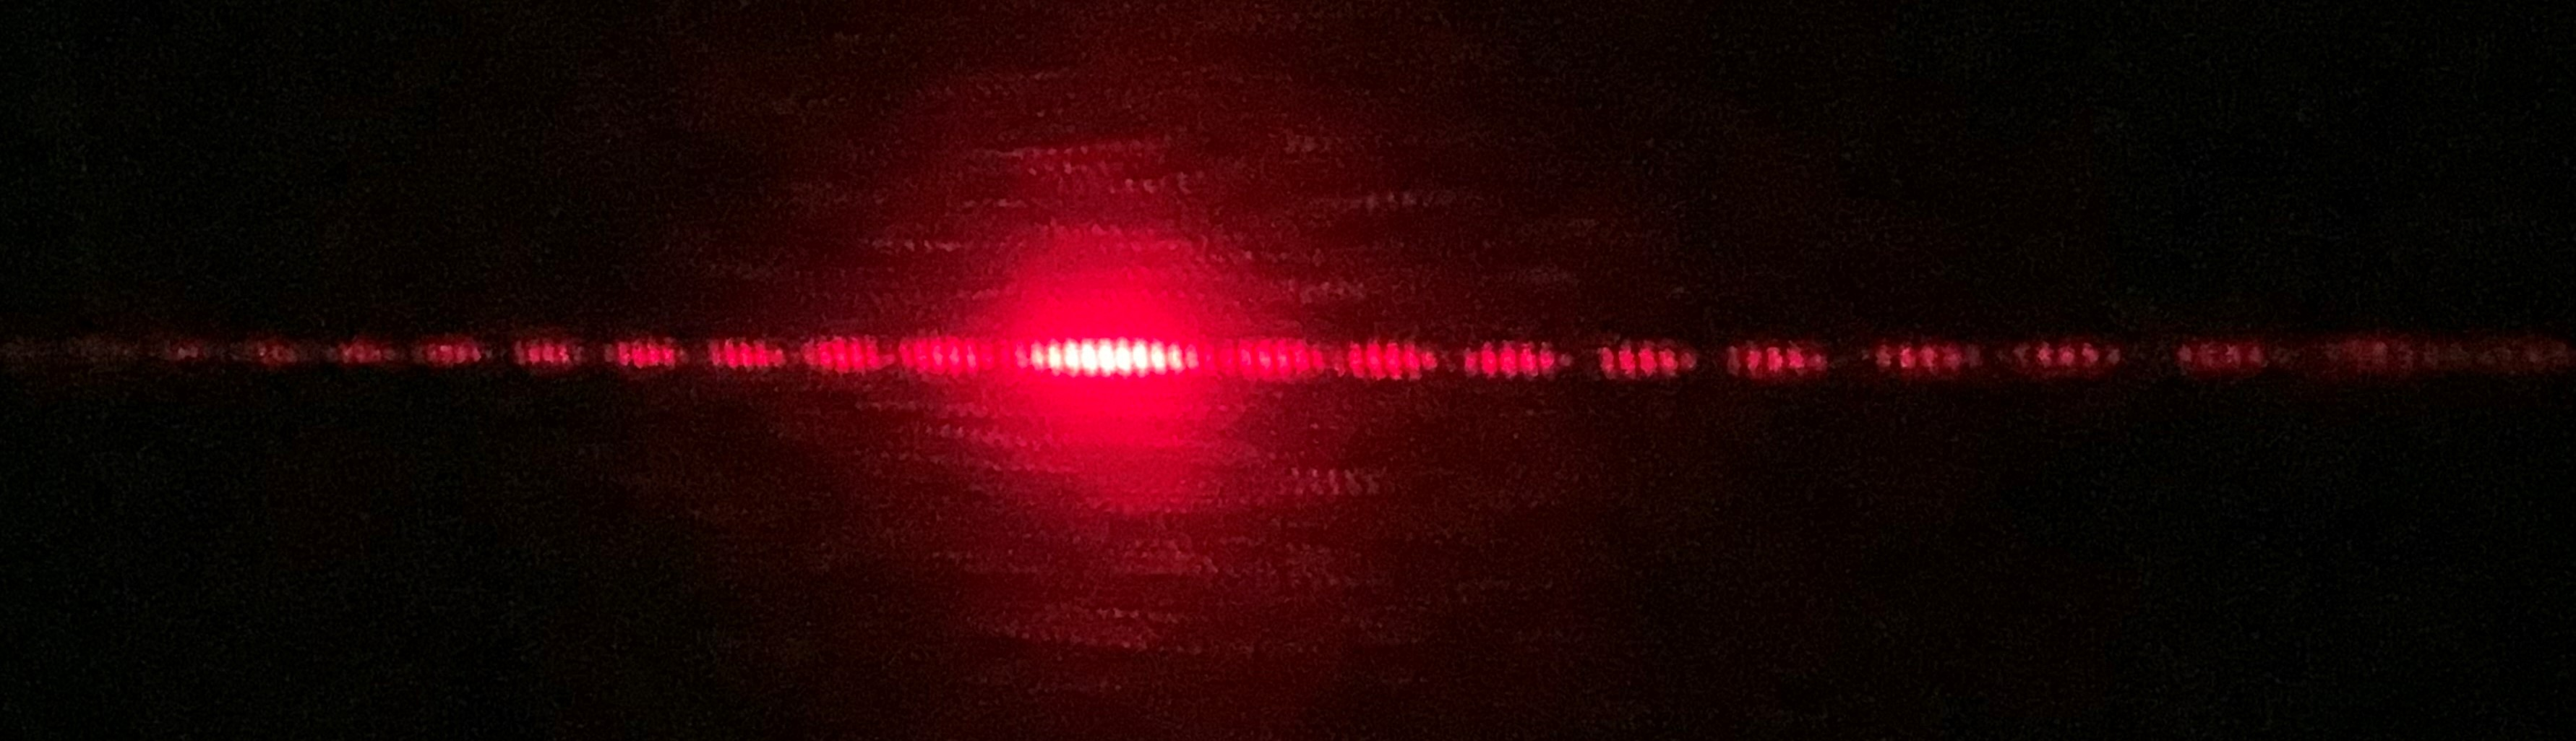
\includegraphics[width=0.7\textwidth]{3_RESUL/08_y_5.jpg}
		\caption{Foto de la rendija}
		\label{fig:A10}
		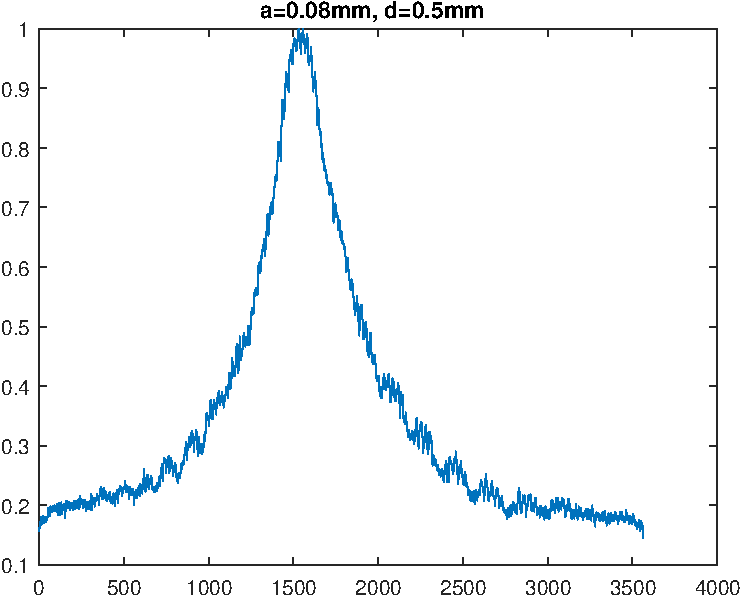
\includegraphics[width=0.7\linewidth,height=7cm]{3_RESUL/08_y_5.pdf}
		\caption{Patrón de irradiancia experimental}
		\label{fig:A11}
		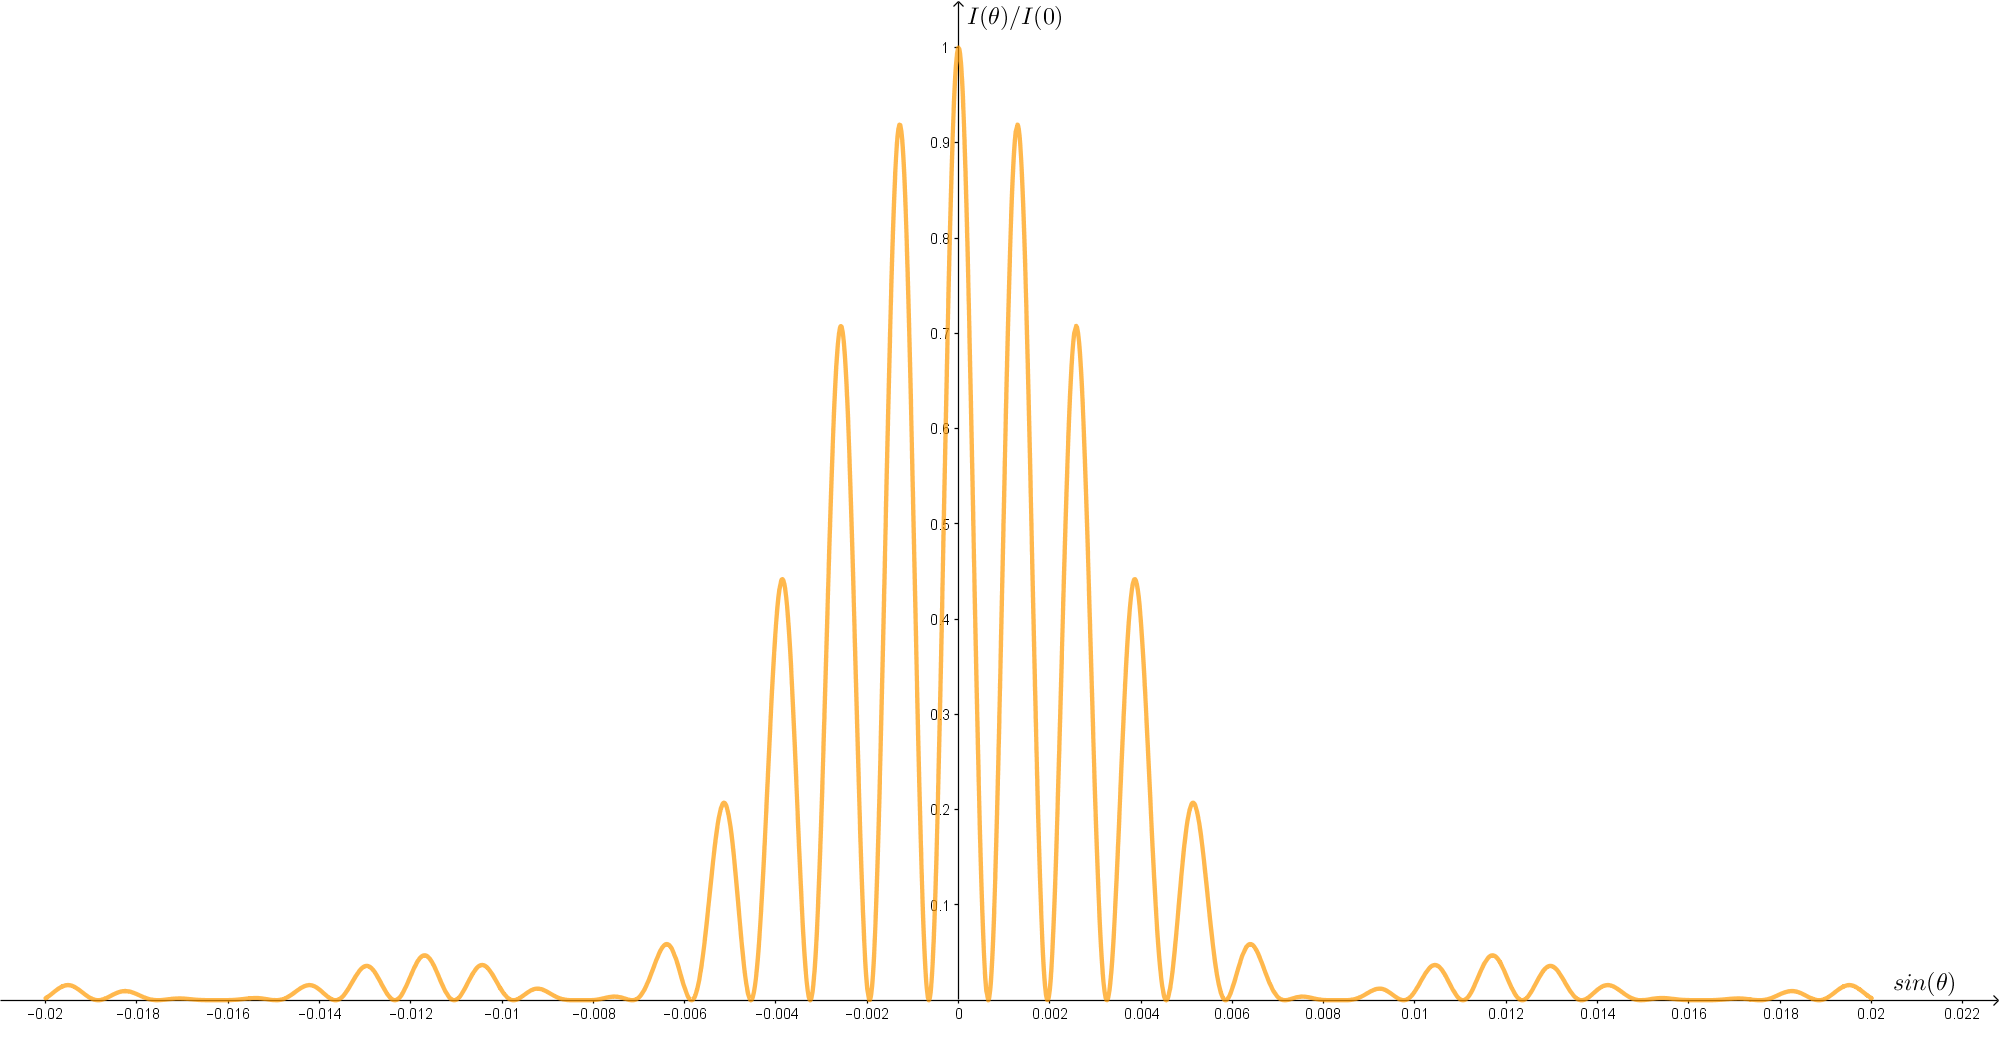
\includegraphics[width=0.7\linewidth,height=7.5cm]{3_RESUL/Irradiancia 4.png}
		\caption{Patrón de irradiancia teórico}
		\label{fig:A12}
		% \caption{Patrones de irradiancia para la rendija indicada}
		% \label{fig:P4}
	\end{figure}
	% )))

% )))
	\newpage

\section{DISCUSIÓN DE RESULADOS Y CONCLUSIONES.} % (((
En esta práctica sobre el experimento de Young, después de haber hecho incidir un láser en cuatro pares de rendijas con anchos y separaciones diferentes cada una, se pudo observar claramente la interferencia formada por la luz en la pantalla, como se muestran en las figuras \ref{fig:A1}, \ref{fig:A4}, \ref{fig:A7} y \ref{fig:A10}, además de que en cada una se obtuvieron patrones de irradiancia distintos en cada rendija. Aunque teóricamente la distancia para cada máximo de interferencia $m$ sólo depende de la distancia de separación $d$ entre cada par de rendijas (como se puede observar en los cálculos de la tabla \ref{tab:disteo}), la tabla \ref{tab:errores} muestra que el cálculo de las diferencias entre las mediciones y los cálculos teóricos son considerables, puesto que se obtuvieron errores relativos que van entre 7.05\% y 23.01\%, aunque al final sigue estando de acuerdo con la fórmula (\ref{eq:altura}), y dicho error se atribuye principalmente a la dificultad de distinción entre los máximos proyectados sobre la pantalla y que produce esta variación con respecto a los valores teóricos obtenidos; para futuras experimentaciones se recomendaría que distintas personas realicen la misma medición sobre tal máximo y promediar las distancias obtenidas para una disminución de este error experimental. \\[2mm]
Sobre el patrón de irradiancia formado por las rendijas, se puede observar respectivamente para cada par de rendijas los patrones observados experimentalmente, cuyo análisis se obtuvo mediante el software Matlab, así como los teóricos, calculados mediante GeoGebra mediante la ecuación (\ref{eq:irradiancia}), los cuales corresponden a las figuras: \ref{fig:A2} y \ref{fig:A3}, \ref{fig:A5} y \ref{fig:A6}, \ref{fig:A8} y \ref{fig:A9}, \ref{fig:A11} y \ref{fig:A12}. En cada par de figuras se puede apreciar, en esencia, la misma forma sobre este patrón normalizado, donde lo único que cambia entre cada par de rendija es lo angosto de la “campana”, y el cual se debe al ancho de cada rendija que hace que la luz se intensifique sobre una superficie mayor o menor según el valor de dicho ancho, y por ende se observan estas diferencias en los patrones de intensidad aunque la distancia de separación entre las rendijas sea la misma. Además, la cantidad de veces en que la función oscila dentro del patrón de difracción depende del patrón de interferencia, el cual, es provocado por el choque de ambas ondas, y que se refleja en la expresión (\ref{eq:irradiancia}). \\[2mm]
Así pues, con todo lo desarrollado se pudo recrear el experimento de Young, el cual nos permite entender a la luz como onda y no sólo como partícula, además de que se pudo obtener la distancia entre distintos máximos de interferencia para distintos pares de rendijas, así como el analizar el patrón de irradiancia para tales rendijas. A mayor anchura de la rendija, menor anchura tendrá el patrón de interferencia, y a mayor distancia de separación entre rendijas, se tendrá una menor distancia entre dos máximos contiguos, en concordancia con la ecuación (\ref{eq:irradiancia}), y comprobado en las secciones \ref{sub:a_bajo_d_bajo}, \ref{sub:a_alto_d_bajo}, \ref{sub:a_bajo_d_alto} y \ref{sub:a_alto_d_alto}. \\[2mm]
% )))

% === REFERENCIAS === (((
\bibliography{Referencias}
\bibliographystyle{unsrt}
% )))

\section{APÉNDICE.} % (((
\subsection{--- Propagación de la Incertidumbre ---}
	La propagación de la incertidumbre para el producto y un cociente están dadas (respectivamente) por
	\begin{align*}
		(x\pm\delta x)(y\pm\delta y)&=x\cdot y\pm\left(|y|\delta x+|x|\delta y \right)\\\\
		\dfrac{x\pm\delta x}{y\pm\delta y}&=\dfrac{x}{y}\pm\left(\dfrac{\delta x}{|y|}+|x|\dfrac{\delta y}{|y|^2}\right)
	\end{align*}
	Para el caso particular en que $ y $ no posee incertidumbre, estas operaciones se simplifican a
	\begin{align*}
		(x\pm\delta x)(y)&=x\cdot y\pm|y|\delta x\\\\
		\dfrac{x\pm\delta x}{y}&=\dfrac{x}{y}\pm\dfrac{\delta x}{|y|}
	\end{align*} 
	\subsection{--- Cálculo teórico de las distancias entre máximos ---}	
	Haciendo uso de la fórmula (\ref{eq:altura}) y los datos experimentales, se obtienen los siguientes cálculos
	\begin{itemize}
		\item Para $ d=0.25mm=0.025cm $
		\begin{align*}
			y_2&=\dfrac{2\cdot (6.5\times10^{-5}cm)\cdot[(90\pm 0.05) cm]}{0.025 cm}=
			\dfrac{(0.0117\pm 6.5\times 10^{-6}) cm^2}{0.025 cm}=
			(0.4680\pm 0.0002)cm\\\\
			y_4&=\dfrac{4\cdot (6.5\times10^{-5}cm)\cdot[(90\pm 0.05) cm]}{0.025 cm}=
			\dfrac{(0.0234\pm1.3\times 10^{-5})cm^2}{0.025 cm}=
			(0.9360\pm0.0005)cm\\
		\end{align*}
		\item Para $ d=0.5mm=0.05cm $
		\begin{align*}
			y_2&=\dfrac{2\cdot (6.5\times10^{-5}cm)\cdot[(90\pm 0.05) cm]}{0.025 cm}=
			\dfrac{(0.0117\pm 6.5\times 10^{-6}) cm^2}{0.05 cm}=
			(0.2340\pm 0.0001)cm\\\\
			y_4&=\dfrac{4\cdot (6.5\times10^{-5}cm)\cdot[(90\pm 0.05) cm]}{0.025 cm}=
			\dfrac{(0.0234\pm1.3\times 10^{-5})cm^2}{0.05 cm}=
			(0.4680\pm0.0002)cm\\
		\end{align*}	
	\end{itemize}
% )))

\end{document}
